\chapter{Implementation}
\label{ch:implementation}

This chapter describes how the design of Chapter~\ref{ch:design} was realised: the implementation platform, the models and algorithms of every stage of the pipeline, and the functional behaviour of the complete system.

\section{Selection of Platform/Programming Language}

\subsection{Choice of Platform and Languages}

\begin{itemize}
  \item \textbf{Raspberry Pi 5 as the edge computer.} A single-board Linux computer runs the complete detection, trust, self-healing and safety pipeline next to the pump, including Isolation Forest scoring and LSTM inference, while exposing the GPIO, SPI and I\textsuperscript{2}C buses that the sensors need. A microcontroller could sample the sensors but could not host the learning models; a remote server could host the models but would put the network inside the safety loop.
  \item \textbf{Python for the edge and the backend.} Python has mature libraries for every part of the system (smbus2 and spidev for the buses, scikit-learn and PyTorch for the models, FastAPI and SQLAlchemy for the service), and one language on both sides allows the edge and the backend to share a single, validated definition of every message.
  \item \textbf{MQTT for messaging.} MQTT is a lightweight publish--subscribe protocol designed for telemetry from constrained devices. Its retained messages and last-will mechanism report device status, and a local broker keeps the system independent of external networks.
  \item \textbf{TypeScript and React for the dashboard.} Static typing catches contract mismatches at build time, and React's component model suits a live display that updates many independent panels every second.
\end{itemize}

\subsection{Repository Organisation}

The system is developed as a single Git repository (a monorepo) with one directory per deployable unit. The edge and the backend share one Python package for the wire contract, so a change to a message format is checked against both sides by the same tests.

\begin{lstlisting}[float=htbp, caption={Top-level structure of the repository}, label={lst:tree}]
SHTAPM/
  edge/        acquisition, drivers, anomaly, trust, pipeline,
               models, actuation, injection, eval, scripts
  backend/     app/api, app/services, app/mqtt, app/ws,
               app/models, app/schemas, alembic, tests
  frontend/    src/app, src/pages, src/features, src/styles
  simulator/   hardware-free telemetry source for development
  infra/       broker configuration, systemd unit
  scripts/     pre-flight self-check, utilities
  docs/        requirements, design and implementation plan
\end{lstlisting}

\subsection{Deployment}

The edge software runs on the Raspberry Pi as the \texttt{systemd} service \texttt{shtapm}, which starts at boot, restarts on failure and releases the relay pin when it stops. The Mosquitto broker runs on the Pi as well, so the edge never depends on another machine to publish. The backend (Uvicorn serving FastAPI) and the dashboard (served by Vite) run on a workstation on the same network. All configuration is read from environment variables: sensor driver selection, sampling rate, window size, broker address, relay pin and polarity, and the location of the persisted baseline and digital-twin bundle. Secrets such as the token-signing key and database password are never stored in the repository.

\subsection{Data Contract}

Every component exchanges the same frozen telemetry frame, defined once as a Pydantic model. Listing~\ref{lst:frame} shows a frame recorded on the rig.

\begin{lstlisting}[float=htbp, caption={A telemetry frame recorded on the bench rig}, label={lst:frame}]
{"device_id": "pump-01",
 "ts": "2026-10-28T07:47:32.955Z",
 "sensors": {"temperature": 27.1, "vibration": 0.0138,
             "pressure": 913.71, "humidity": 49.1,
             "gas": 148.34, "current": 0.0},
 "sample_seq": 55}
\end{lstlisting}

A decision message carries, for each window, the anomaly flag, severity, attribution (\texttt{none}, \texttt{fault} or \texttt{attack}), a reason, the trust score of every channel, the set of isolated channels and the value substituted for each. A ledger message carries an event type and its payload.

\section{Model Implementation \& Algorithm}

\subsection{Acquisition and Sensor Health}

The sampler reads every driver once per second and assembles a frame. A driver that fails to answer does not stop the frame: its last good value is held, and the channel is reported dead only after 5~s of continuous failure, so that the brief dropouts of the DHT22 when the motor starts are absorbed. Two driver-level safeguards were added after faults observed on the bench: a DHT22 reader that has failed continuously for 10~s re-opens the device, and an ADXL335 reading at either rail of the 10-bit converter (0 or 1023 counts) is treated as a failed read, because it indicates a loose connection rather than a real acceleration.

\subsection{Sensor Drivers and Signal Conversion}

Each driver converts the raw output of its device into engineering units.

\paragraph{Vibration (ADXL335 through MCP3008).} The MCP3008 returns a 10-bit count $n \in [0, 1023]$ per axis with a 3.3~V reference, and the ADXL335 has a nominal sensitivity of $S = 0.330$~V/$g$ at a 3.3~V supply, so one count corresponds to
\begin{equation}
\Delta a = \frac{V_{\mathrm{ref}}}{1024\, S} = \frac{3.3}{1024 \times 0.330} \approx 9.77 \times 10^{-3}~g.
\end{equation}
The first successful read establishes an at-rest baseline $(n_x^0, n_y^0, n_z^0)$, which absorbs each axis's zero-$g$ offset and the static gravity component, and vibration is reported as the magnitude of the deviation from it:
\begin{equation}
v = \Delta a \sqrt{(n_x - n_x^0)^2 + (n_y - n_y^0)^2 + (n_z - n_z^0)^2}.
\end{equation}
This makes vibration a relative quantity that is zero for a still motor in any mounting orientation.

\paragraph{Current (INA219).} The INA219 measures the voltage across a 0.1~$\Omega$ shunt in series with the motor supply. For a maximum expected current of 5~A, the current resolution and the calibration register value are
\begin{equation}
I_{\mathrm{LSB}} = \frac{5}{32767} \approx 1.526 \times 10^{-4}~\mathrm{A}, \qquad
\mathrm{Cal} = \left\lfloor \frac{0.04096}{I_{\mathrm{LSB}}\, R_{\mathrm{shunt}}} \right\rfloor = 2684,
\end{equation}
and the current is the signed register value multiplied by $I_{\mathrm{LSB}}$.

\paragraph{Pressure (BMP280).} The BMP280 is triggered in forced mode for one conversion per sample, and its raw temperature and pressure words are converted with the manufacturer's integer compensation formulas and the twelve calibration coefficients read from the device at start-up.

\paragraph{Temperature and humidity (DHT22).} The DHT22 transmits a 40-bit frame over a single-wire protocol containing humidity, temperature and a checksum. Reads that fail the checksum or time out are reported as failed reads and handled by the hold-last-value logic described above.

\paragraph{Gas (MQ-135).} The analogue output of the MQ-135 can exceed the converter's 3.3~V range, so it passes through a resistor divider of 10~k$\Omega$ and 13~k$\Omega$ into MCP3008 channel~3, and the driver restores the sensor voltage with the divider ratio $(10 + 13)/13 = 1.769$. The channel is reported in volts: converting the voltage to a gas concentration in parts per million requires a clean-air calibration of the individual sensor, and no unvalidated concentration is reported.

Both converter-based channels reject readings at either rail of the converter, and the DHT22 reader is re-opened after 10~s of continuous failure, as described in the previous section.

\subsection{Baseline Recording and Calibration}

The detector, the consistency and reliability evidence, the channel flag policy and the vibration bands are all fitted on a recording of clean operation of the actual rig. The procedure used for the deployed baseline was:

\begin{enumerate}
  \item Record telemetry on the Pi for about 50 minutes while switching the motor on and off by hand at irregular intervals, so that both motor states and many transitions are represented.
  \item A few minutes into the recording, and again later, run a recording check that splits the frames by motor state using the current (idle below 0.05~A, running above 0.3~A) and reports, per five-minute block, the median idle and running vibration, frame gaps and missing values. The check fails if idle vibration exceeds 0.5~$g$ (the sensor has moved), if running vibration is not at least twice the idle level, or if frames are missing for more than 3~s.
  \item Fit the baseline on the first 80\% of the recording and score the remaining 20\% as a hold-out: because the hold-out is clean, every alarm in it is a false alarm. The check also reports the median clean trust per channel, which must exceed 0.7 so that an isolated channel can always be released, and the coverage of the learned vibration bands.
  \item Install the fitted baseline on the Pi and restart the edge service, which loads it at start-up.
\end{enumerate}

A first 70-minute recording was rejected by this procedure because the accelerometer shifted on the first motor run, which made idle and running vibration indistinguishable; the recording check was introduced so that such a problem is caught within minutes rather than after the full recording.

\subsection{Preprocessing}

For each channel, the last $W = 30$ samples form a window $\mathbf{x} = (x_1, \dots, x_W)$, and a new window is produced with every frame. The preprocessing chain consists of a sliding median filter of odd kernel $m$, a first-order low-pass filter
\begin{equation}
y_t = a\,x_t + (1 - a)\,y_{t-1}, \qquad 0 < a \leq 1,
\end{equation}
and a per-window min--max normalisation
\begin{equation}
\tilde{x}_i = \frac{x_i - \min_j x_j}{\max_j x_j - \min_j x_j},
\end{equation}
with a flat window ($\max = \min$) mapped to zeros. Both filters are configurable; the deployed configuration uses $m = 1$ and $a = 1$ (identity), and the detector is calibrated on windows prepared in exactly the same way.

\subsection{Anomaly Detection with Isolation Forest}

Isolation Forest~\cite{liu2008iforest} builds an ensemble of random binary trees, each grown on a random sub-sample of $\psi$ training points by choosing a random feature and a random split value at every node. An anomalous point is isolated close to the root. With $h(\mathbf{x})$ the path length of point $\mathbf{x}$ in one tree, the anomaly score is
\begin{equation}
s(\mathbf{x}, \psi) = 2^{-\frac{\mathbb{E}[h(\mathbf{x})]}{c(\psi)}}, \qquad c(\psi) = 2H(\psi - 1) - \frac{2(\psi - 1)}{\psi},
\end{equation}
where $H(i) \approx \ln i + 0.5772$ is the harmonic number and $c(\psi)$ is the average path length of an unsuccessful search in a binary search tree, used for normalisation.

In SHTAPM each $30 \times 6$ window is flattened into one 180-dimensional observation, and a single forest of 100 trees is fitted on the windows of the recorded clean baseline. Raw scores are not thresholded directly. Instead, the scores of the clean windows are stored, and the \emph{severity} of a new window is the empirical cumulative distribution value of its score within them:
\begin{equation}
\mathrm{sev}(\mathbf{x}) = \frac{\left|\{\, j : s_j^{\mathrm{clean}} \leq s(\mathbf{x}) \,\}\right|}{N_{\mathrm{clean}}} \in [0, 1].
\end{equation}
A window is flagged when $\mathrm{sev} \geq 0.90$. By construction about 10\% of clean windows are flagged; the detector is deliberately sensitive, and the trust engine and the physics rule decide which flags matter. The window-level flag is localised to channels by comparing each channel's window variance with that channel's own baseline distribution: a channel is flagged when its variance falls in the lowest or highest 10\% of its clean distribution. This two-sided test catches both a spike or a constant spoof (abnormally low normalised variance) and noisy behaviour (abnormally high variance).

\subsection{Trust Engine}
\label{sec:trust}

Every channel carries a Beta-reputation state~\cite{josang2002beta} $(\alpha, \beta)$, initialised to $\alpha_0 = \beta_0 = 1$, with trust
\begin{equation}
T = \frac{\alpha}{\alpha + \beta} \in [0, 1].
\end{equation}
Each window supplies an evidence value $g \in [0, 1]$ built from three independent terms.

\paragraph{Consistency $c$.} For each sample, $z_i = (x_i - \mu)/\sigma$ with the channel's baseline mean and standard deviation; the window statistic is $r = \sqrt{\tfrac{1}{W}\sum_i z_i^2}$, and $c = 1 - F_r(r)$, where $F_r$ is the empirical distribution of $r$ over the clean windows. A window that looks like typical clean data scores near 0.5; an extreme window scores near 0.

\paragraph{Physical correlation $k$.} $k = 1$ unless the operating-state rule (Section~\ref{sec:attribution}) finds current and vibration describing an impossible motor state, in which case the suspect channel receives $k = 0$ (both channels when the rule cannot tell which one moved). Channels without a physical partner always receive $k = 1$.

\paragraph{Historical reliability $h$.} An exponentially weighted record of past outcomes,
\begin{equation}
h_t = \gamma\, h_{t-1} + (1 - \gamma)\, o_t, \qquad \gamma = 0.95,\; h_0 = 1,
\label{eq:h}
\end{equation}
where $o_t = 1$ when the channel was not flagged in window $t$ and $0$ otherwise. Its half-life is about 13 windows.

The evidence and the update are
\begin{align}
g &= 0.4\,c + 0.3\,k + 0.3\,h, \\
\alpha_t &= \lambda\, \alpha_{t-1} + g, \qquad \beta_t = \lambda\, \beta_{t-1} + (1 - g), \qquad \lambda = 0.7.
\label{eq:betaupdate}
\end{align}
The forgetting factor $\lambda$ gives the trust an effective memory of $1/(1 - \lambda) \approx 3.3$ windows. Under constant evidence $g$ the state converges to $\alpha^{*} = g/(1 - \lambda)$ and $\beta^{*} = (1 - g)/(1 - \lambda)$, so that
\begin{equation}
T^{*} = \frac{\alpha^{*}}{\alpha^{*} + \beta^{*}} = g,
\end{equation}
which means the trust score settles exactly at the level of the evidence: it is bounded, interpretable and free of drift. Channels are classified as \textbf{Trusted} ($T \geq 0.7$), \textbf{Suspicious} ($0.4 \leq T < 0.7$) or \textbf{Malicious} ($T < 0.4$).

Figure~\ref{fig:trustdyn} illustrates the dynamics of these equations for an idealised evidence profile: typical clean evidence ($c = 0.5$, $k = 1$), then 45 windows of fully adverse evidence ($c = 0$, $k = 0$, flagged), then clean evidence again. Trust falls from Trusted to Malicious within three windows, but returns to Trusted only after 21 clean windows, because $h$ recovers slowly. This asymmetry is intentional: a sensor that has lied must earn its trust back.

\begin{figure}[htbp]
\centering
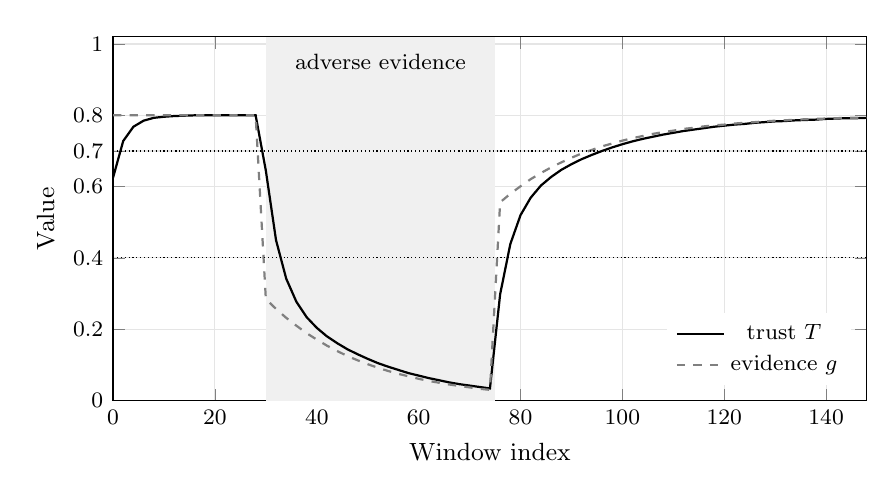
\begin{tikzpicture}
\begin{axis}[
  width=0.92\textwidth, height=6.2cm,
  xlabel={Window index}, ylabel={Value},
  xmin=0, xmax=148, ymin=0, ymax=1.02,
  ytick={0,0.2,0.4,0.6,0.7,0.8,1},
  legend style={at={(0.98,0.04)}, anchor=south east, font=\footnotesize, draw=none, fill=white},
  tick label style={font=\footnotesize}, label style={font=\small},
  grid=major, grid style={gray!20}]
\fill[gray!12] (axis cs:30,0) rectangle (axis cs:75,1.02);
\node[font=\footnotesize, anchor=north] at (axis cs:52.5,1.0) {adverse evidence};
\addplot[thick, black] coordinates {(0,0.625) (2,0.728) (4,0.768) (6,0.785) (8,0.793) (10,0.796) (12,0.798) (14,0.799) (16,0.8) (18,0.8) (20,0.8) (22,0.8) (24,0.8) (26,0.8) (28,0.8) (30,0.645) (32,0.45) (34,0.342) (36,0.277) (38,0.234) (40,0.204) (42,0.18) (44,0.161) (46,0.144) (48,0.13) (50,0.117) (52,0.105) (54,0.095) (56,0.086) (58,0.077) (60,0.07) (62,0.063) (64,0.057) (66,0.051) (68,0.046) (70,0.042) (72,0.038) (74,0.034) (76,0.298) (78,0.439) (80,0.52) (82,0.569) (84,0.603) (86,0.627) (88,0.647) (90,0.663) (92,0.677) (94,0.689) (96,0.7) (98,0.71) (100,0.719) (102,0.727) (104,0.734) (106,0.74) (108,0.746) (110,0.751) (112,0.756) (114,0.76) (116,0.764) (118,0.768) (120,0.771) (122,0.774) (124,0.776) (126,0.779) (128,0.781) (130,0.783) (132,0.784) (134,0.786) (136,0.787) (138,0.788) (140,0.79) (142,0.791) (144,0.792) (146,0.792) (148,0.793)};
\addlegendentry{trust $T$}
\addplot[thick, dashed, gray] coordinates {(0,0.8) (28,0.8) (30,0.285) (32,0.257) (34,0.232) (36,0.21) (38,0.189) (40,0.171) (42,0.154) (44,0.139) (46,0.125) (48,0.113) (50,0.102) (52,0.092) (54,0.083) (56,0.075) (58,0.068) (60,0.061) (62,0.055) (64,0.05) (66,0.045) (68,0.041) (70,0.037) (72,0.033) (74,0.03) (76,0.556) (78,0.58) (80,0.601) (82,0.621) (84,0.638) (86,0.654) (88,0.668) (90,0.681) (92,0.693) (94,0.703) (96,0.713) (98,0.721) (100,0.729) (102,0.736) (104,0.742) (106,0.748) (108,0.753) (110,0.757) (112,0.762) (114,0.765) (116,0.769) (118,0.772) (120,0.774) (122,0.777) (124,0.779) (126,0.781) (128,0.783) (130,0.785) (132,0.786) (134,0.788) (136,0.789) (138,0.79) (140,0.791) (142,0.792) (144,0.793) (146,0.793) (148,0.794)};
\addlegendentry{evidence $g$}
\addplot[thin, densely dotted, black, domain=0:148] {0.7};
\addplot[thin, densely dotted, black, domain=0:148] {0.4};
\end{axis}
\end{tikzpicture}
\caption{Response of the trust update rule to an idealised evidence profile, computed from Equations~\eqref{eq:h}--\eqref{eq:betaupdate}; dotted lines mark the 0.7 and 0.4 band limits}
\label{fig:trustdyn}
\end{figure}

\begin{lstlisting}[float=htbp, language=Python, caption={Beta-reputation state update (\texttt{edge/trust/beta.py})}, label={lst:beta}]
def combine_g(c: float, k: float, h: float) -> float:
    return W_CONSISTENCY * c + W_CORRELATION * k + W_RELIABILITY * h

def update(self, g: float) -> float:
    self.alpha = self.forgetting * self.alpha + g
    self.beta = self.forgetting * self.beta + (1.0 - g)
    return self.alpha / (self.alpha + self.beta)
\end{lstlisting}

\subsection{Physics-Based Attribution}
\label{sec:attribution}

A pump motor is either running or idle, and both its supply current and its vibration reflect that state. Each of the two sensors is therefore an independent witness of the motor state. The operating-state rule classifies each channel from the \emph{median} of its raw window, so that impulsive events such as a tap or a one-sample glitch cannot flip the state:
\begin{equation}
\mathrm{state}(\mathbf{x}) =
\begin{cases}
\textsc{idle}, & \mathrm{median}(\mathbf{x}) \leq b_{\mathrm{idle}}, \\
\textsc{running}, & \mathrm{median}(\mathbf{x}) \geq b_{\mathrm{run}}, \\
\textsc{unclear}, & \text{otherwise.}
\end{cases}
\end{equation}
For current, $b_{\mathrm{idle}} = 0.05$~A and $b_{\mathrm{run}} = 0.3$~A. Vibration depends on how the sensor is mounted, so its bands are learned from the steady windows of the clean baseline: $b_{\mathrm{idle}}$ is 1.5 times the 99.9th percentile of the idle window medians, and $b_{\mathrm{run}}$ lies midway between $b_{\mathrm{idle}}$ and the 5th percentile of the running window medians. On the deployed baseline this gives $b_{\mathrm{idle}} = 0.142$~$g$ and $b_{\mathrm{run}} = 0.314$~$g$. The gap between the bands acts as hysteresis: a window inside it gives no verdict, so motor transitions never produce a violation.

When one channel reports \textsc{idle} and the other \textsc{running}, the machine described by the data is physically impossible and one reading must be false. The suspect is the channel whose state changed most recently while the other stayed constant: a motor that really starts or stops moves both channels together, whereas a single falsified channel moves alone. Algorithm~\ref{alg:attribution} summarises the procedure. An anomaly is attributed as an \emph{attack} on the suspect when physics is violated, and as a \emph{fault} otherwise; when several labels compete, the priority is attack, then fault, then none.

\begin{algorithm}[H]
\caption{Operating-state attribution for one window}
\label{alg:attribution}
\begin{algorithmic}[1]
\Require raw windows $\mathbf{x}_{I}$ (current) and $\mathbf{x}_{V}$ (vibration); channel flags $F$; previous states $s_I^{-}, s_V^{-}$
\Ensure attribution label and suspect channel
\State $s_I \gets \mathrm{state}(\mathbf{x}_I)$, \; $s_V \gets \mathrm{state}(\mathbf{x}_V)$
\If{$\{s_I, s_V\} = \{\textsc{idle}, \textsc{running}\}$}
  \If{$s_I \neq s_I^{-}$ \textbf{and} $s_V = s_V^{-}$} \State suspect $\gets$ current
  \ElsIf{$s_V \neq s_V^{-}$ \textbf{and} $s_I = s_I^{-}$} \State suspect $\gets$ vibration
  \Else \State suspect $\gets$ both
  \EndIf
  \State \Return (\textsc{attack}, suspect, ``physics violation'')
\ElsIf{any channel in $F$ is flagged}
  \State \Return (\textsc{fault}, flagged channels, ``physically consistent anomaly'')
\Else
  \State \Return (\textsc{none}, --, --)
\EndIf
\end{algorithmic}
\end{algorithm}

The rule covers the physically coupled pair of channels on this rig. Temperature, humidity, pressure and gas have no physical partner on the bench and can only be attributed as faults; extending physical coupling to them requires a process with the corresponding relationships, such as discharge pressure in a real pump.

\subsection{Isolation and Self-Healing with an LSTM Digital Twin}

A channel enters isolation when its trust falls below 0.4 and leaves it when trust returns to 0.7; the Suspicious band in between prevents oscillation. While a channel is isolated, its reading is removed from fusion and replaced by a reconstruction from the digital twin, and the dashboard marks the value as \textsc{virtual}.

The twin is a single-layer, unidirectional LSTM~\cite{hochreiter1997lstm}. For each time step $t$ of the 30-sample window, the input $\mathbf{u}_t$ concatenates the six channel values, with the isolated channel set to zero, and a six-element one-hot mask that names the missing channel. The LSTM computes
\begin{align}
\mathbf{i}_t &= \sigma(\mathbf{W}_i \mathbf{u}_t + \mathbf{U}_i \mathbf{h}_{t-1} + \mathbf{b}_i), &
\mathbf{f}_t &= \sigma(\mathbf{W}_f \mathbf{u}_t + \mathbf{U}_f \mathbf{h}_{t-1} + \mathbf{b}_f), \nonumber\\
\mathbf{o}_t &= \sigma(\mathbf{W}_o \mathbf{u}_t + \mathbf{U}_o \mathbf{h}_{t-1} + \mathbf{b}_o), &
\tilde{\mathbf{c}}_t &= \tanh(\mathbf{W}_c \mathbf{u}_t + \mathbf{U}_c \mathbf{h}_{t-1} + \mathbf{b}_c), \nonumber\\
\mathbf{c}_t &= \mathbf{f}_t \odot \mathbf{c}_{t-1} + \mathbf{i}_t \odot \tilde{\mathbf{c}}_t, &
\mathbf{h}_t &= \mathbf{o}_t \odot \tanh(\mathbf{c}_t),
\end{align}
and the reconstruction is $\hat{y} = \mathbf{w}^{\top} \mathbf{h}_{30} + b$. Inputs and target are expressed on a fixed z-score scale computed from the clean training data, so the output is converted back to engineering units exactly.

The deployed twin reconstructs motor current from vibration, the channel that is physically coupled to it; the ambient channels are excluded from its input because they carry no information about current on this rig. It has 32 hidden units and was trained with the Adam optimiser (learning rate 0.01, 30 epochs, mean-squared-error loss) on three bench recordings, with the last 15\% of each recording held out. No training window spans two recordings or a gap in time. Training is performed on the workstation with PyTorch, and the trained weights, scale and residual statistics are saved together as one bundle that the edge loads at start-up, so a model can never be used with a scale it was not trained on.

Substitution is bounded. An uncertainty value $u = \min(t_s/60, 1)$ grows with the elapsed substitution time $t_s$ in seconds; when $u$ exceeds 0.8 (after 48~s) the self-healing layer raises an internal signal that the budget is nearly exhausted, and after 60~s of continuous substitution the self-healing layer escalates to a Safe Pump-Stop. A second escalation path compares the live reading with the twin's reconstruction and escalates when their divergence exceeds a threshold. It is implemented and tested but disabled in the deployed configuration: on clean held-out data, a 3$\sigma$ threshold would have produced false escalations in 4.5\% of windows, which is not acceptable for an action that stops the plant.

\subsection{Safety Supervisor}

The safety supervisor is the only component allowed to switch the pump relay. It acts on four causes: an operator command, a self-healing escalation, a dry-run signature (pump commanded on, past a 5~s spin-up grace, with the current inside the dry-run band for three consecutive frames), and a watchdog that fires when no healthy frame has arrived for 10~s while the pump runs. Every autonomous stop \emph{latches}: the pump stays off until an administrator restarts it through a confirmation dialog. The edge forces the relay off at start-up and at shutdown, and the service manager releases the relay pin after a crash, so every failure mode ends with the pump stopped. Figure~\ref{fig:safetysm} shows the state machine.

\begin{figure}[htbp]
\centering
\begin{tikzpicture}[
  st/.style={draw, rounded corners=8pt, minimum width=3.0cm, minimum height=1.0cm, align=center, font=\small, fill=white},
  tr/.style={-{Stealth[length=2.2mm]}, thick},
  tl/.style={font=\scriptsize, align=center}]
  \node[st] (off) at (0,0) {\textsc{off}};
  \node[st] (run) at (6.5,0) {\textsc{running}};
  \node[st] (lat) at (3.25,-3.2) {\textsc{latched off}};
  \draw[tr] (off) to[bend left=18] node[tl, above]{operator start} (run);
  \draw[tr] (run) to[bend left=18] node[tl, below]{operator stop} (off);
  \draw[tr] (run) -- node[tl, below right]{self-heal escalation,\\dry run, watchdog} (lat);
  \draw[tr] (lat) -- node[tl, below left]{administrator\\confirmed restart} (off);
  \draw[tr] (-2.6,0) -- node[tl, above]{start-up} (off);
\end{tikzpicture}
\caption{State machine of the safety supervisor}
\label{fig:safetysm}
\end{figure}

Relay commands travel on their own MQTT topic, separate from scenario injections, so an injected test scenario can never reach the relay. Each transition is reported by the edge as an actuation status (relay state, cause, reason, latched flag and whether a physical relay is attached), and the backend chains every transition into the ledger.

\subsection{Tamper-Evident Audit Ledger}

Safety-relevant events are appended to a hash chain~\cite{haber1991timestamp}. For block $n$ with timestamp $\tau_n$ and payload $P_n$,
\begin{align}
\mathrm{ph}_n &= \mathrm{SHA256}\big(\mathrm{canon}(P_n)\big), \\
H_n &= \mathrm{SHA256}\big(n \,\|\, \tau_n \,\|\, \mathrm{ph}_n \,\|\, H_{n-1}\big), \qquad H_{-1} = 0^{64},
\end{align}
where $\mathrm{canon}$ serialises the payload as JSON with sorted keys and no insignificant whitespace, so that the same payload always produces the same digest, and $\|$ denotes concatenation. Modifying any field of block $n$ changes $\mathrm{ph}_n$ or $H_n$ and breaks the link stored in block $n+1$. Algorithm~\ref{alg:verify} shows the verifier, and Table~\ref{tab:ledgerevents} the events that are chained.

\begin{algorithm}[H]
\caption{Ledger verification}
\label{alg:verify}
\begin{algorithmic}[1]
\Require blocks $B_0, \dots, B_N$ of one device in index order
\Ensure valid, or the index of the first broken block
\State $e \gets 0^{64}$
\For{$n = 0$ \textbf{to} $N$}
  \State \textbf{if} $B_n.\mathrm{ph} \neq \mathrm{SHA256}(\mathrm{canon}(B_n.P))$ \textbf{then return} broken at $n$
  \State \textbf{if} $B_n.\mathrm{prev} \neq e$ \textbf{then return} broken at $n$
  \State \textbf{if} $B_n.H \neq \mathrm{SHA256}(n \,\|\, B_n.\tau \,\|\, B_n.\mathrm{ph} \,\|\, B_n.\mathrm{prev})$ \textbf{then return} broken at $n$
  \State $e \gets B_n.H$
\EndFor
\State \Return valid
\end{algorithmic}
\end{algorithm}

\begin{table}[htbp]
\centering
\caption{Events recorded in the audit ledger}
\label{tab:ledgerevents}
\small
\begin{tabularx}{\textwidth}{@{}l X@{}}
\toprule
\textbf{Event type} & \textbf{Recorded when} \\
\midrule
\texttt{trust\_drop} & A channel's trust crosses below the Malicious limit, with the edge's attribution \\
\texttt{isolate} & A channel is isolated and digital-twin substitution begins \\
\texttt{released\_from\_isolation} & An isolated channel's trust recovers and the real reading is restored \\
\texttt{recover} & A channel returns to the Trusted band \\
\texttt{safe\_stop} & The supervisor stops the pump autonomously \\
\texttt{relay\_command} & An administrator requests a relay change \\
\texttt{relay\_on}, \texttt{relay\_off} & The edge reports a relay transition \\
\texttt{inject} & An administrator starts or cancels a test scenario \\
\texttt{config\_update} & An administrator changes a threshold \\
\bottomrule
\end{tabularx}
\end{table}

\subsection{Scenario Injection}

To evaluate the system with known ground truth, and to let an administrator rehearse incidents live, the edge can transform one channel's readings for a set duration. Eight transforms are implemented (Table~\ref{tab:injections}). In the live path the injection is applied inside the edge, after acquisition and before detection, so it travels the identical path that a real falsified reading would take.

\begin{table}[htbp]
\centering
\caption{Implemented fault and attack injections ($x_t$: true reading, $t$: samples since onset)}
\label{tab:injections}
\small
\begin{tabularx}{\textwidth}{@{}l l X@{}}
\toprule
\textbf{Injection} & \textbf{Class} & \textbf{Injected value} \\
\midrule
Gradual drift & Fault & $x_t + r\,t$ \\
Sudden spike & Fault & $x_t + A$ for the active samples \\
Stuck sensor & Fault & value frozen at onset \\
Bias injection & Attack & $x_t + b$ \\
Ramp injection & Attack & $x_t + r\,t$ \\
Replay & Attack & the channel's own earlier recording \\
Constant spoof & Attack & a constant value $v$ \\
Adaptive stealth & Attack & $x_t + \mathrm{clip}(r\,t, -\delta, \delta)$, kept below a residual bound $\delta$ \\
\bottomrule
\end{tabularx}
\end{table}

\subsection{Backend Services}

The backend subscribes to the edge's telemetry, decision, status and actuation topics. Each message is validated against the contract and written to the database off the hot path. Telemetry frames are additionally fanned out immediately to connected dashboards over a WebSocket, so the live trends move with every sample; decisions, alerts, the live physics state and the relay state are served through REST endpoints that the dashboard polls every one to five seconds (the live state every second and decisions every two). On top of the stored data the backend maintains:

\begin{itemize}
  \item \textbf{Alerts}: one alert per incident, raised at the moments the ledger records them: a trust drop (critical, labelled attack or fault from the edge's attribution), a Safe Pump-Stop (critical) and a dead sensor (warning). Operators acknowledge alerts from the dashboard.
  \item \textbf{Device condition}: a rollup that reports \emph{critical} on a latched Safe Pump-Stop, attacks in a majority (5) of the last 10 decisions, or an isolated channel under a fresh attack; \emph{warning} on an isolated channel or faults and attacks in a majority of the last 10; and \emph{healthy} otherwise.
  \item \textbf{Live state}: the edge's motor-state reading and the twin's reconstructed values, for display.
  \item \textbf{Sensor health}: which channels are currently dead and since when.
\end{itemize}

\paragraph{Security.} Passwords are hashed with bcrypt. Login returns a signed JSON Web Token valid for 15 minutes and a refresh token valid for 7 days that is rotated on use and revoked on logout. Every REST endpoint and the WebSocket validate the token; the WebSocket closes with code 4401 for an invalid token and 4403 for a device the user may not access. Table~\ref{tab:rbac} shows the role permissions and Table~\ref{tab:api} the principal endpoints.

\begin{table}[htbp]
\centering
\caption{Role-based access control}
\label{tab:rbac}
\small
\begin{tabularx}{\textwidth}{@{}X c c c@{}}
\toprule
\textbf{Capability} & \textbf{Operator} & \textbf{Analyst} & \textbf{Administrator} \\
\midrule
View control room, sensors, decisions and history & Yes & Yes & Yes \\
View and acknowledge alerts & Yes & Yes & Yes \\
View, verify and export the audit ledger & -- & Yes & Yes \\
Inject test scenarios & -- & Yes & Yes \\
Start or stop the pump & -- & -- & Yes \\
Thresholds, devices, users and system health & -- & -- & Yes \\
\bottomrule
\end{tabularx}
\end{table}

\begin{table}[htbp]
\centering
\caption{Principal REST and WebSocket endpoints}
\label{tab:api}
\small
\begin{tabularx}{\textwidth}{@{}l l X@{}}
\toprule
\textbf{Method} & \textbf{Path} & \textbf{Purpose} \\
\midrule
POST & \texttt{/api/auth/\{login, refresh, logout\}} & Authentication \\
GET & \texttt{/api/devices/\{id\}/readings} & Telemetry history \\
GET & \texttt{/api/devices/\{id\}/decisions} & Decision history with trust and attribution \\
GET & \texttt{/api/devices/\{id\}/live-state} & Motor state and twin values \\
GET & \texttt{/api/devices/\{id\}/sensor-health} & Dead-sensor status \\
GET, PATCH & \texttt{/api/devices/\{id\}/thresholds} & Detection thresholds (administrator) \\
POST & \texttt{/api/devices/\{id\}/inject} & Start a test scenario (analyst, administrator) \\
GET, POST & \texttt{/api/devices/\{id\}/relay} & Relay state and commands (administrator) \\
GET & \texttt{/api/ledger/\{id\}} & Ledger blocks (analyst, administrator) \\
POST & \texttt{/api/ledger/\{id\}/verify} & Chain verification \\
GET & \texttt{/api/ledger/\{id\}/export} & Ledger export \\
GET, POST & \texttt{/api/alerts}, \texttt{/\{id\}/ack} & Alerts and acknowledgement \\
GET & \texttt{/api/system/health} & Broker, sample rate and latency (administrator) \\
WS & \texttt{/ws?token=\ldots\&device\_id=\ldots} & Live telemetry stream \\
\bottomrule
\end{tabularx}
\end{table}

\subsection{Dashboard}

The dashboard is a React and TypeScript single-page application designed on the principles of ANSI/ISA-101~\cite{isa101}: displays are calm and neutral during normal operation, colour is reserved for abnormal conditions, and every status is conveyed by text as well as by colour. Table~\ref{tab:pages} lists its pages. Two display rules prevent a single noisy window from alarming the operator: the control room shows a fault only when it holds 5 of the last 10 decisions, and a channel that has sent nothing for 10~s is shown as \textsc{no data} rather than with a stale value.

\begin{table}[htbp]
\centering
\caption{Dashboard pages}
\label{tab:pages}
\small
\begin{tabularx}{\textwidth}{@{}l X@{}}
\toprule
\textbf{Page} & \textbf{Content} \\
\midrule
Control room & Live status of all six channels, motor-state physics panel, trust per channel, incident timeline and current verdict \\
Sensor detail & Opened from any channel: live trend, trust history, statistics, health, and the twin's value when substituted \\
Devices & Monitored pumps with their condition and a plain-language explanation of it \\
Device & Device information, scenario injection and the pump relay panel \\
Decisions & Decision log with trust timeline, attribution and reason \\
History & Stored telemetry over a selectable period \\
Alerts & Active and acknowledged alerts with severity and reason \\
Ledger & Hash-chained events and one-click chain verification \\
System & Live architecture view, broker status, sample rate and end-to-end latency \\
Users & Account and role management (administrator) \\
Settings & Connection and display preferences; current detection thresholds \\
\bottomrule
\end{tabularx}
\end{table}

\subsection{Prognosis and Response-Policy Modules}
\label{sec:impl-prognosis-rl}

Two further components of the original design were implemented as modules and verified by unit tests, but are not part of the deployed decision path.

\textbf{Prognosis.} An LSTM prognosis network and its full data pipeline were built against the public PRONOSTIA (FEMTO) bearing run-to-failure dataset~\cite{nectoux2012pronostia}, including the input representation, data-quality rules and remaining-useful-life targets. A remaining-life prediction for the pump needs run-to-failure data from the pump itself, which a bench rig cannot produce; the deployed system therefore reports condition (healthy, warning, critical) from the rollup described above and never presents a remaining-life estimate.

\textbf{Response policy.} The reinforcement-learning layer provides the state vector (machine health, anomaly flag, six trust scores and failure estimate), the action set (continue, reduce weight, isolate sensor, trigger alert, Safe Pump-Stop), a reward that penalises false isolation, missed critical faults and downtime, a simulation environment with synthetic degradation, a deep Q-network training harness and a fallback gate. The deployed system runs the deterministic rule-based policy described in this chapter, which the requirements specify as the fail-safe fallback (FR-RL4). Choosing the reward weights is a policy decision about the acceptable trade-off between false isolation and downtime, and training the learned policy is left as future work.

\section{Functional Description of Modules}

The complete behaviour of the system for one cycle is as follows.

\begin{enumerate}
  \item \textbf{Start-up.} The edge loads the persisted clean baseline, fits the Isolation Forest, the channel flag policy, the consistency provider and the vibration bands on it, loads the twin bundle, forces the relay off and connects to the broker. If no baseline exists, it warms up on live data instead and logs that it has done so.
  \item \textbf{Sampling.} Once per second the sampler reads all drivers, applies any active test injection and publishes the frame.
  \item \textbf{Decision.} The newest 30 frames form a window. The pipeline scores it, updates $c$, $k$, $h$ and the trust of every channel, and runs the attribution rule.
  \item \textbf{Self-healing.} The isolation tracker compares each trust score with the 0.4 and 0.7 limits; isolated channels are substituted by the twin and their substitution clocks are advanced or reset.
  \item \textbf{Safety.} The supervisor checks escalation, dry-run and watchdog conditions and switches the relay if required.
  \item \textbf{Publication.} The decision (flag, severity, attribution, reason, trust, isolation set, substituted values) and any actuation change are published.
  \item \textbf{Backend.} The backend stores the messages, raises alerts and ledger blocks on edge-triggered transitions, updates the device condition and streams the telemetry to the dashboard over the WebSocket.
  \item \textbf{Presentation.} The dashboard redraws the live trends with every frame and refreshes the verdict, trust and physics panels from the REST endpoints within one to two seconds of the decision.
\end{enumerate}
